\section{Working with Markov Chains [18pts Grad / 6\% Bonus for Undergrads]}



\subsection{Markov Mechanics [6pts Grad / 2\% Bonus for Undergrads]}
Suppose we have a sequence of random variables $\{X_t\}_{t \in \mathbb{Z}^{\ge 0}}$ that take on values from the set $\mathcal{S} \coloneq \{1, 2, \dots, n\}$ (where $n$ is just some positive integer). We could think of the value of $X_t$ as the state of some system at time $t$ and we could think of $\mathcal{S}$ as the set of all possible states the system could be in. Naturally, we'd like to compute $P(X_t = x_t)$, the probability that the system is at state $x_t \in \mathcal{S}$ at time $t$. If we make the assumption that this is modelling a physical system, we can conclude the current state is dependent on the past, but not on the future. Furthermore, we suppose the system can take any value from $\mathcal{S}$ at every time $t$. Thus, we can say:
\begin{equation} \label{eq:longeq}
    P(X_t = x_t) = \sum_{x_{t - 1} \in \mathcal{S}}\sum_{x_{t - 2} \in \mathcal{S}} \dots \sum_{x_{0} \in \mathcal{S}}P(X_t = x_t \mid X_{t - 1} = x_{t - 1}, \dots, X_0 = x_0)P(X_{t - 1} = x_{t - 1}, \dots, X_0 = x_0).
\end{equation}
As it stands now, computing $P(X_t = x_t)$ for a fixed $x_t$ would require us to add $n^t$ terms and know all of the different $n^t$ conditional probability distributions, which becomes intractible for relatively small values of $n$ and $t$. To simplify, we can make an assumption known as the \textbf{first-order Markov assumption}:
$$P(X_t = x_t \mid X_0 = x_0, \dots, X_{t - 1} = x_{t - 1}) = P(X_t = x_t \mid X_{t - 1} = x_{t - 1}),$$
for any $t \geq 1$. We've assumed that the current state is dependent only on the most recent state, and not the entire history. Our sequence $\{X_t\}_{t \in \mathbb{N}}$ is now called a \textbf{Markov chain}. You can verify that \eqref{eq:longeq}, under this assumption, becomes
$$P(X_t = x_t) = \sum_{x_{t - 1} \in S} P(X_t = x_t \mid X_{t - 1} = x_{t - 1})P(X_{t - 1} = x_{t - 1}).$$
With this assumption, we only need to know the conditional probabilities for a single timestep, $P(X_{t} = i \mid X_{t - 1} = j)$ for all $i, j \in \mathcal{S}$, and the distribution over the initial states, $P(X_0 = x_0)$ for any $x_0 \in \mathcal{S}$. These conditional probabilities are known as \textbf{transition probabilities}. It's also common to model these transition probabilities as constant over time, that is, $P(X_{t} = i \mid X_{t - 1} = j) = P(X_{q} = i \mid X_{q - 1} = j)$ for any $q, t \geq 1$ and $i, j \in \mathcal{S}$. To organize the transition probabilities, we can define a matrix $A \in \mathbb{R}^{n \times n}$ such that $A_{ij} \coloneq P(X_{t} = i \mid X_{t - 1} = j)$\footnote{You'll have to use 1-indexing if you want this to align with our definition $\mathcal{S} \coloneq \{1, 2, \dots, n\}$.}. Because these are probabilities over all $\mathcal{S}$, all entries will be non-negative, and the columns will sum to 1:
$$ \forall j \; \left[ \sum_{k = 1}^n A_{kj} = 1 \right] \qquad \text{and} \qquad \forall i,j\; \left[ A_{ij} \geq 0 \right] $$
Matrices with these properties are called \textbf{stochastic matrices}. If we let $\vec{x}_0 \coloneq \begin{bmatrix}P(X_0 = 1) & \dots & P(X_0 = n)\end{bmatrix}^\top$, we can simulate a time-evolution of the system simply by multiplying by the matrix, $\vec{x_1}=A\vec{x_0}$\footnote{It may be instructive to work out a single element of $\vec{x_1}$ symbolically, and confirm that it does correctly evaluate the sum rule using the transition probabilities to get the probability of the system at the next timestep.}. More generally, the $i$-th entry of $\vec{x}_t \coloneq A\vec{x}_{t - 1}$ is $P(X_t = i)$. Crucially, since we assumed that the transition probabilities are constant over time, we don't even need a recurrence relation, we can just repeatedly multiply $\vec{x_0}$ by $A$, $\vec{x}_t = A^t\vec{x}_0$.

\begin{enumerate}[label=\alph*.]
    \item Given an $n \times n$ stochastic matrix $A$, \emph{prove} that 1 is always an eigenvalue of $A$. [3pts Grad / 1\% Bonus for Undergrads]

    \item Let's interpret that result. Given an eigenvalue $\lambda$ of $A$, we know that there must exist an eigenvector $\vec{v}$ such that $A\vec{v} = \lambda\vec{v}$. With $\lambda=1$, we know further that $A\vec{v}=\vec{v}$. Interpreting $A$ as a transformation, $\vec{v}$ is unaffected by this transformation. When such a $\vec{v}$ is a \textit{probability vector} (i.e., a vector whose entries are non-negative and sum to 1), then interpreting $\vec{v}$ as a distribution over our states $\mathcal{S}$ means that this distribution over the states is unaffected by time-evolution. Thus, it's called a \textit{steady-state vector}. When the state of our system has approached a steady-state vector with $A\vec{v}=\vec{v}$, then our belief of the state of the system doesn't change.

    \smallskip Given the stochastic matrix $$A = \begin{bmatrix}1/2 & 2/3 \\ 1/2 & 1/3\end{bmatrix},$$
    find all steady-state vectors of the corresponding Markov chain. Remember to normalize your result to a probability vector. \emph{Show your work. Round your final result to 3 decimal places.} [3pts Grad / 1\% Bonus for Undergrads]
\end{enumerate}
\newpage



\subsection{Application to PageRank [12pts Grad / 4\% Bonus for Undergrads]}
The Google PageRank algorithm is a classic application of Markov chains. The main objective is ranking webpages by their importance, which we roughly take to mean the proportion of time a user spends on a webpage as they surf the Web. Each webpage is a state, and the transition probabilities dictate how a user moves between the webpages that are hyperlinked on the current webpage. To satisfy some regularity conditions, slight adjustments are made to the stochastic matrix $A$ (i.e., the final stochastic matrix we get isn't going to only be made up of the transition probabilities as was explained in the previous part):

\begin{itemize}
    \itemsep0em
    \item If there exists a column of $A$ with only a single entry being 1, replace the whole column of $A$ with $1/n$, where $n$ is the number of webpages in total, to get a new matrix $A'$.
    
    \item We then compute the Google matrix $G$, where
    $$G \coloneq \alpha A' + (1 - \alpha)K,$$
    $0 < \alpha < 1$, and $K$ is the matrix with all entries equal to $1/n$. The idea is that sometimes a websurfer will close the tab and start a new search at a random site.
    
    \item $G$ is the stochastic matrix that represents an appropriate Markov chain for modelling our problem. 
\end{itemize}
Now, $G$ must have a unique steady state $\vec{x}^*$, that is, for any valid initial distribution $\vec{x}_0$, we have that
$$\vec{x}^* \coloneq \lim_{k \to \infty} \vec{x}_k = \lim_{k \to \infty} G^k\vec{x}_0 \implies G\vec{x}^* = \vec{x}^*$$

Suppose we have 3 webpages on the Web. The following graph represents the different transition probabilities between the webpages.

\begin{figure}[!h]
    \centering
    \begin{tikzpicture}[thin, node distance=43mm, main/.style = {draw, circle, minimum size=1cm}, lbl/.style={midway, fill=white, font=\small}]
        \node[main] (1) {$1$};
        \node[main] (2) [right of=1] {$2$};
        \draw[bend left=20, ->] (1) to node[lbl] {\sfrac{1}{4}} (2);
        \draw[bend left=20, ->] (2) to node[main] (3) [midway, below=0.5cm] {$3$} node[lbl] {\sfrac{1}{10}} (1);
        \draw[->] (1) to [out=150, in=210, looseness=4.5] node[lbl] {\sfrac{1}{2}} (1);
        \draw[->] (2) to [out=30, in=330, looseness=4.5] node[lbl] {\sfrac{4}{5}} (2);
        \draw[->] (1) to [out=270, in=180] node[lbl] {\sfrac{1}{4}} (3);
        \draw[->] (2) to [out=270, in=0] node[lbl] {\sfrac{1}{10}} (3);
        \draw[->] (3) to [out=300, in=240, looseness=4.5] node[lbl] {1} (3);
    \end{tikzpicture}
\end{figure}

For the sake of cleanliness, we've excluded any edges with a weight of 0, but all other edges should be present and interpretable as transition probabilities. For example, we see here that $P(X_{t} = 2 \mid X_{t - 1} = 1) = \frac{1}{4}$.

You'll be applying PageRank to this tiny web. From user surveying, we've found that $\alpha=0.8$ is a good choice for our modelling purposes.

\begin{enumerate}[label=\alph*.]
    \item Construct the base stochastic matrix, $A$. [1.5pts Grad / 0.5\% Bonus for Undergrads] % no work required to be shown
    \item Construct $G$. \emph{Show your work.} [6pts Grad / 2\% Bonus for Undergrads]
    \item Find the unique steady-state vector of $G$. \emph{Show your work.} [3pts Grad / 1\% Bonus for Undergrads]
    \item Order the webpages by how frequently a user would visit the webpages as they surf the Web indefinitely. [1.5pts Grad / 0.5\% Bonus for Undergrads] % no work required to be shown
\end{enumerate}
\begin{warningbox}
    Your work will be easier to evaluate if you do not round intermediate results. You should represent all numbers appearing in your work for this question as fractions or integers.
\end{warningbox}
\newpage
